
\vspace{-5pt}
\section{Experiments}
\label{sec:expr}
\vspace{-5pt}
\subsection{Experimental Setups}
\label{sec:exp_setups}

In our experimental setup, \anno{we train nine language models ranging from 122M to 70B parameters in total, which share the same data distribution and architecture, with the training data scaled proportionally to their sizes.} We show the detailed training configurations and recipe in Appendix~\ref{append:setting}.

% \noindent\textbf{Downstream evaluation sets.}
For evaluation, we adopt the following widely used benchmarks, including GSM8K \citep{cobbe2021training}, MATH \citep{hendrycks2021measuring}, BBH \citep{suzgun2023challenging}, TriviaQA \citep{joshi2017triviaqa},
MBPP \citep{austin2021program}, AGIEval \citep{zhong2023agieval},
DROP \citep{dua2019drop}, MMLU-pro \citep{wang2024mmlu}. 
All models are evaluated in a few-shot in-context learning manner, and we aligned our evaluation setups with LLaMa3~\citep{dubey2024llama}.We evaluate the proposed COD performance scaling for LLMs against existing approaches on multiple public benchmarks. Using eight smaller language models as known information, we estimate the downstream task performance of a pretrained LLM with 70B parameters. 

\subsection{Prediction Experiments}
\label{subsec:Prediction_Experiments}
We compare COD against four representative prediction methods:
\begin{enumerate}[leftmargin=2em]
\item Loss-intermediate~\citep{chen2024scaling}: First predicts the target LLM's final training or validation loss, then estimates downstream task metrics based on the relationship between smaller models' evaluation metrics and their losses.
\item \camera{End-to-end(exp)}~\citep{xiao2024densing}: Directly extrapolates large model metrics from smaller model evaluation set metrics using \camera{exponential-based} performance scaling laws.
\item \camera{End-to-end(passrate)}~\citep{achiam2023gpt,hu2023predicting}: A variant of end-to-end method, which estimates large model passrates from smaller model passrates. We conduct 100 trials per evaluation set for smaller models to enhance reliability and report absolute prediction error on the passrate metric.
\item \camera{End-to-end(BNSL)}~\citep{caballero2022broken}: Decomposes the end-to-end mapping into a multi-segment power-law framework.
\end{enumerate}

\begin{table*}[!t]
\small
\setlength{\tabcolsep}{1.8pt} % Keep this if column spacing is critical
\centering
\caption{Absolute prediction error (\%) on evaluation sets for predicting the performance of the 70B model. Errors < 2\% are considered accurate (green), while errors > 5\% are considered invalid (red). $\downarrow$ indicates lower is better.}
\begin{tabular}{c|cc|cccccccc}
\toprule
\multirow{2}{*}{Method} & \multicolumn{2}{c|}{Overall Metrics} & \multicolumn{8}{c}{Individual Task Sets} \\
\cmidrule(lr){2-3} \cmidrule(lr){4-11}
& Mean$\downarrow$ & Max$\downarrow$ & GSM8k & MATH & BBH & TriviaQA & MBPP & AGIEval & DROP & MMLU-pro \\
\midrule
Loss-intermediate & 5.29 & 9.39 & \redhl{9.39} & \redhl{6.95} & 2.33 & \redhl{5.81} & \redhl{5.52} & \greenhl{1.41} & \redhl{5.37} & \redhl{5.55} \\
End-to-end\camera{(exp)} & 3.10 & 6.00 & 4.00 & 3.86 & \greenhl{0.64} & \greenhl{0.68} & \greenhl{1.75} & \redhl{6.00} & 4.11 & 3.72 \\
\camera{End-to-end(passrate)} & 5.02 & 8.80 & \redhl{6.71} & \redhl{8.80} & 3.51 & 4.00 & \redhl{7.34} & \redhl{6.78} & \greenhl{0.26} & 2.74 \\
\camera{End-to-end(BNSL)} & 5.17 & 13.05 & 4.23 & \redhl{5.88} & \redhl{13.05} & \redhl{5.86} & 2.55 & \greenhl{0.82} & \greenhl{1.53} & \redhl{7.42} \\
\midrule
COD (w/o mapping) & 2.24 & 5.26 & 4.70 & \greenhl{0.50} & 2.91 & \greenhl{1.98} & \greenhl{0.89} & \redhl{5.26} & \greenhl{1.08} & \greenhl{0.57} \\
% COD (Complete) & \textbf{1.63} & \textbf{2.38} & 2.23 & \greenhl{1.28} & \greenhl{1.77} & \greenhl{1.64} & 2.19 & 2.38 & \greenhl{0.23} & \greenhl{1.35} \\
COD (Complete) & \textbf{1.55} & \textbf{2.68} & 2.68 & \greenhl{0.79} & \greenhl{0.47} & \greenhl{1.97} & 2.42 & \greenhl{1.64} & \greenhl{1.05} & \greenhl{1.39} \\
\bottomrule
\end{tabular}
\label{tab:baseline_comparison}
\vspace{-10pt}
\end{table*}

We also evaluate two variants of our COD approach to validate the benefits of its components:
\begin{enumerate}[leftmargin=2em]
    \item COD (w/o mapping): Performs difficulty-based KMeans clustering, extrapolates per cluster, and aggregates metrics without subset-to-full mapping.
    \item COD (Complete): Our full proposed multi-stage approach, including clustering, predictable cluster filtering, subset extrapolation, and subset-to-full mapping.
\end{enumerate}

Comparative results are shown in \cref{tab:baseline_comparison}. Prediction accuracy is measured by the absolute error between predicted and actual performance. We report mean and max prediction errors across all evaluation sets, as well as errors for individual sets. Our complete COD approach significantly outperforms existing methods in both mean (\camera{1.55\%}) and maximum (\camera{2.68\%}) prediction errors, offering reliable guidance for large model training. \camera{Although baseline methods achieve acceptable performance on partial datasets, their large prediction errors on other datasets severely compromise their overall reliability.}
% While baselines perform well on some sets, their substantial errors on others undermine overall credibility.

\begin{figure}[!t]
\vspace{-5pt}
    \centering
    % Assuming minipage setup is for layout, keeping it.
    \begin{minipage}{0.24\textwidth}
        \centering
        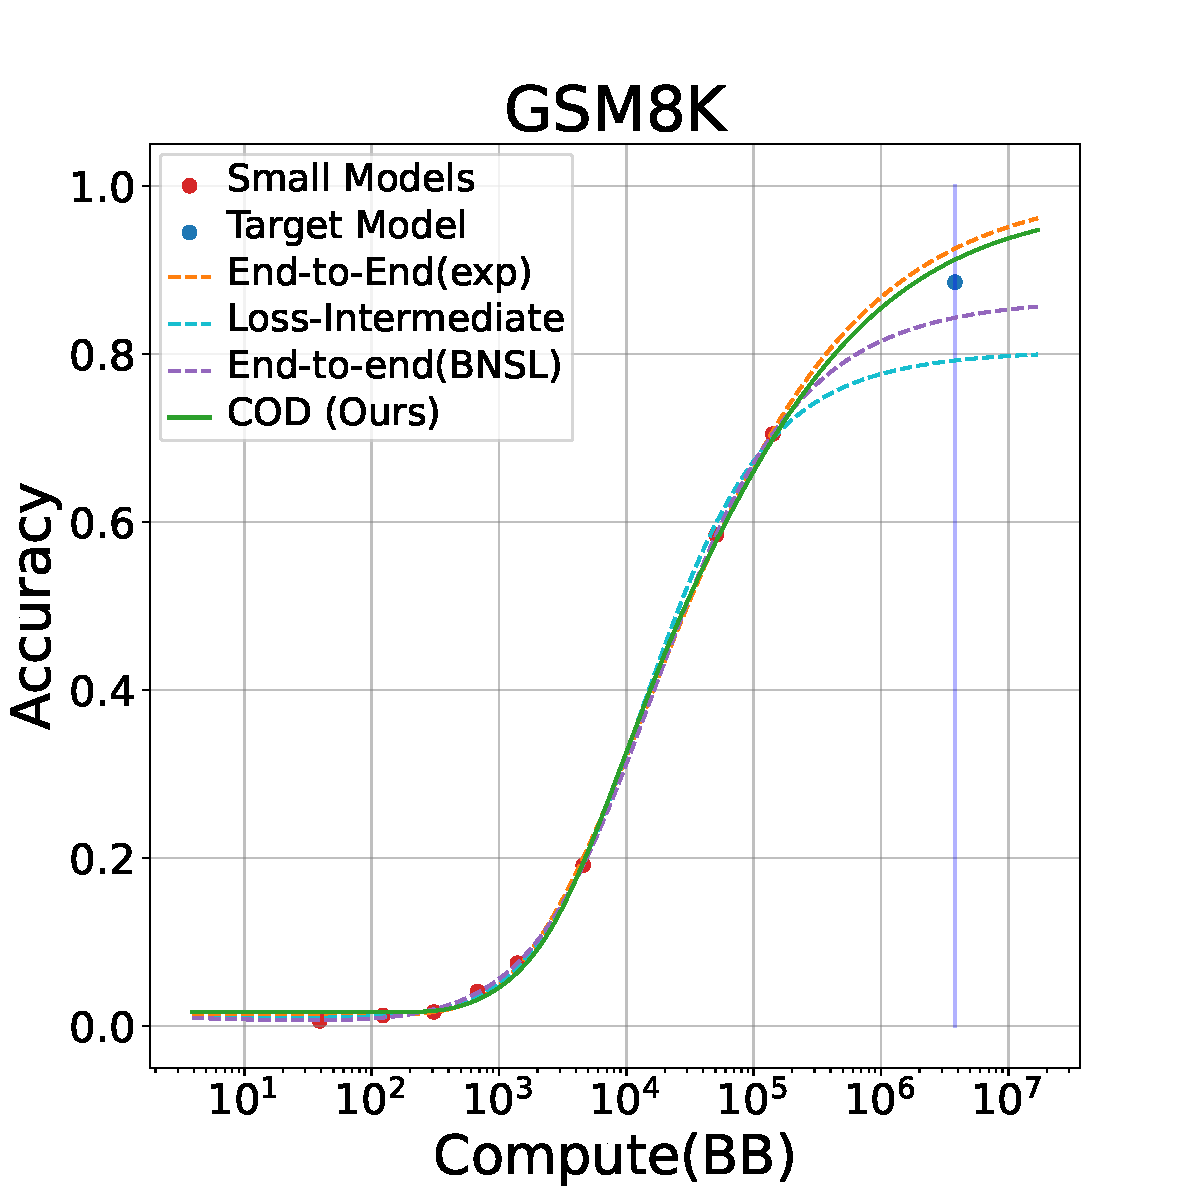
\includegraphics[width=\textwidth]{figures/experiments/perf_compute/GSM8K.pdf}
    \end{minipage}
    \begin{minipage}{0.24\textwidth}
        \centering
        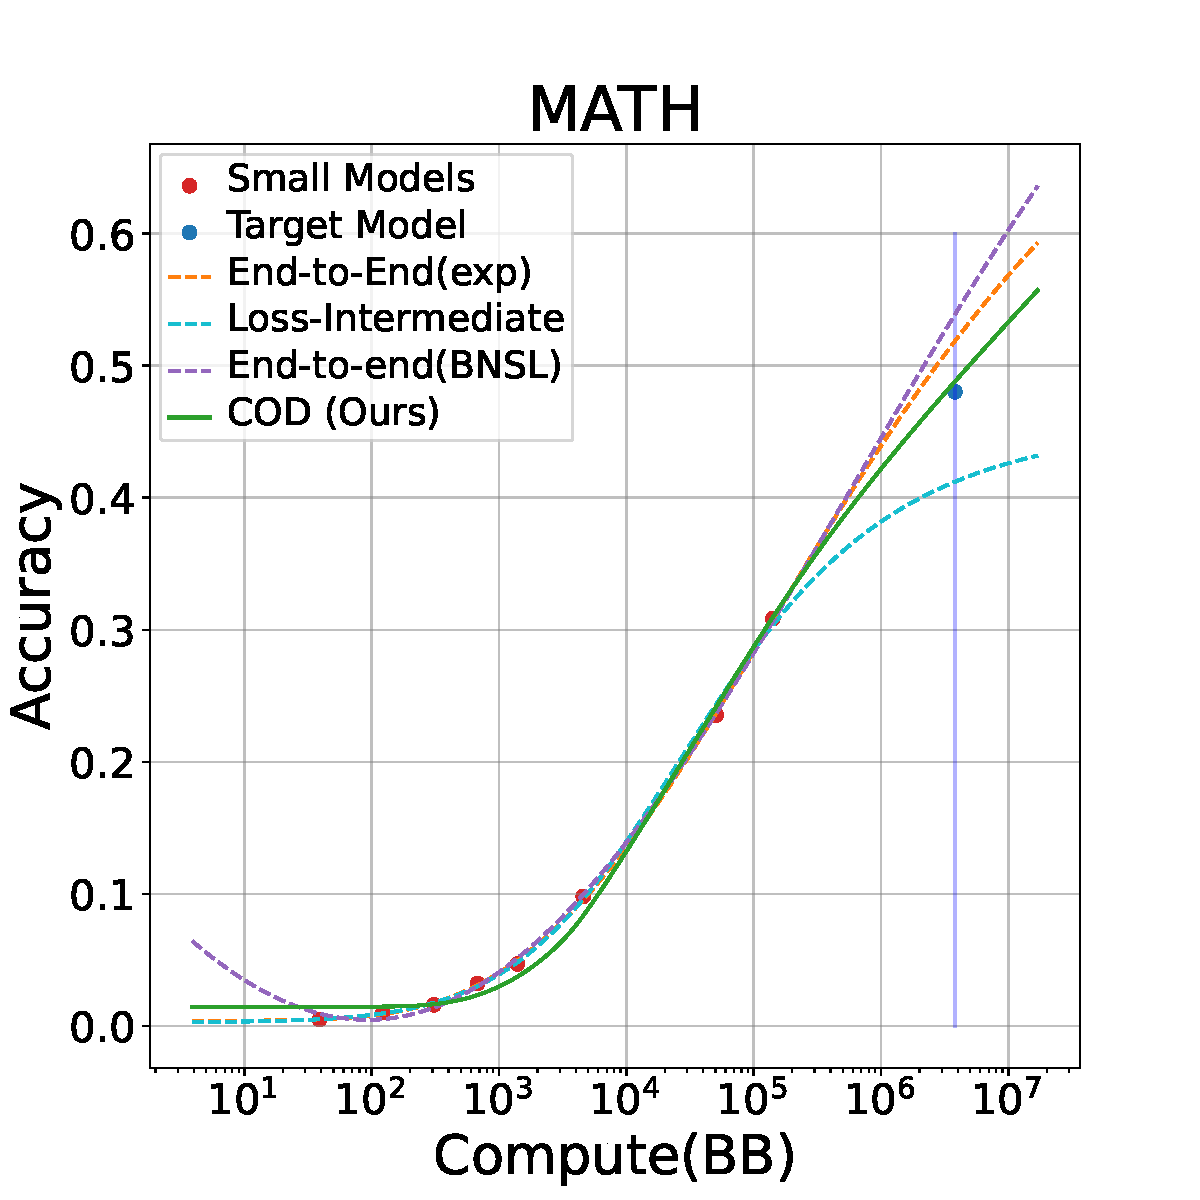
\includegraphics[width=\textwidth]{figures/experiments/perf_compute/MATH.pdf}
    \end{minipage}
    \begin{minipage}{0.24\textwidth}
        \centering
        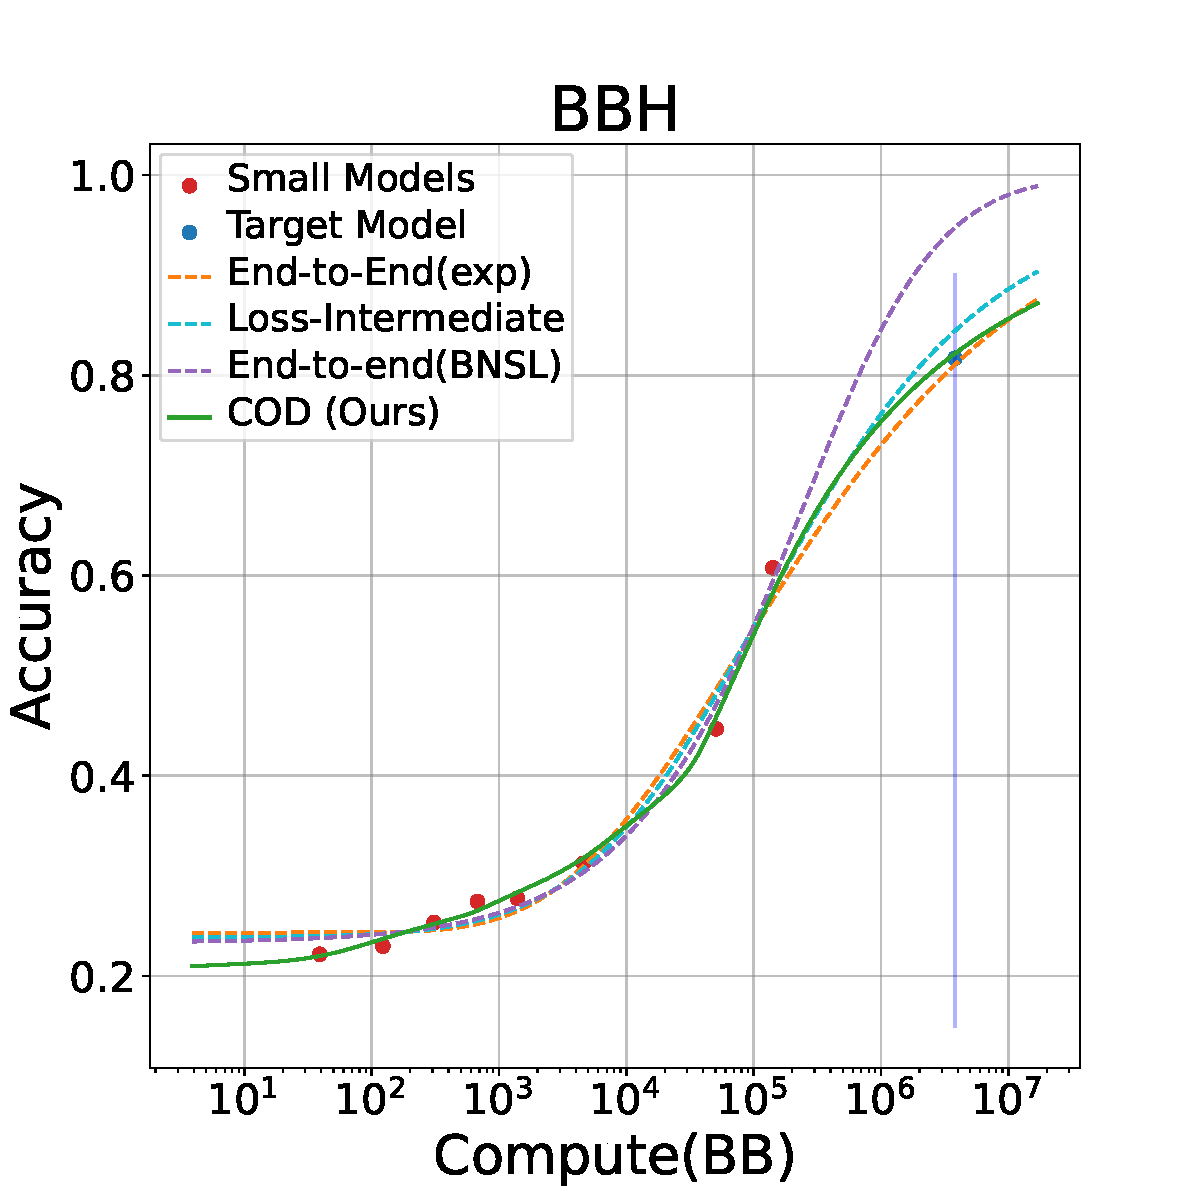
\includegraphics[width=\textwidth]{figures/experiments/perf_compute/BBH.pdf}
    \end{minipage}
    \begin{minipage}{0.24\textwidth}
        \centering
        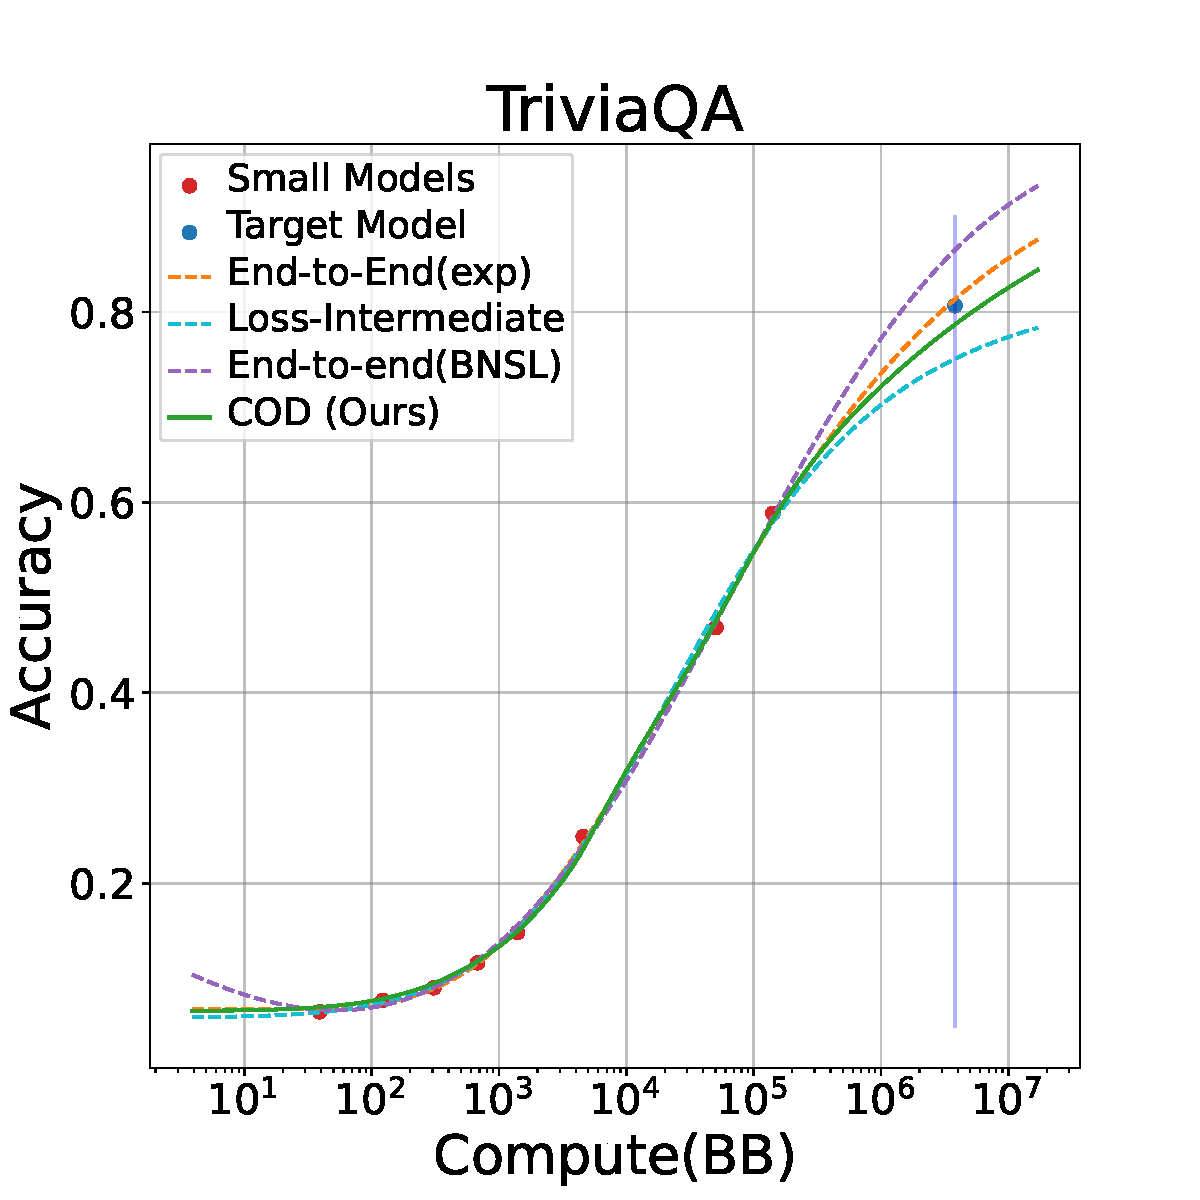
\includegraphics[width=\textwidth]{figures/experiments/perf_compute/TRIVIAQA.pdf}
    \end{minipage}

    \begin{minipage}{0.24\textwidth}
        \centering
        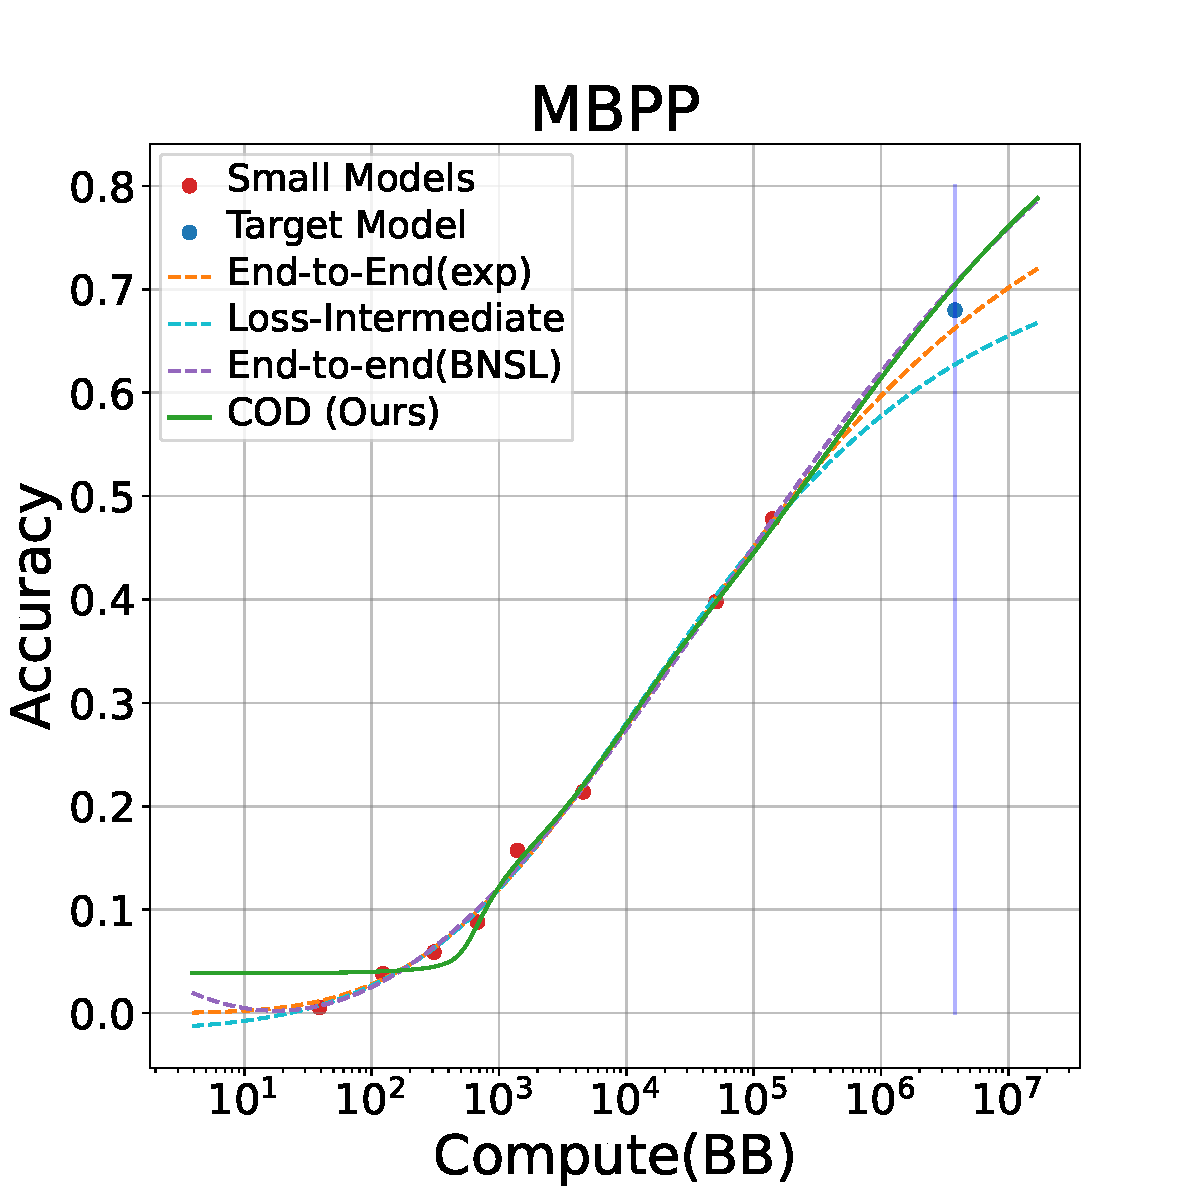
\includegraphics[width=\textwidth]{figures/experiments/perf_compute/MBPP.pdf}  % 替换为实际文件名
    \end{minipage}
    \begin{minipage}{0.24\textwidth}
        \centering
        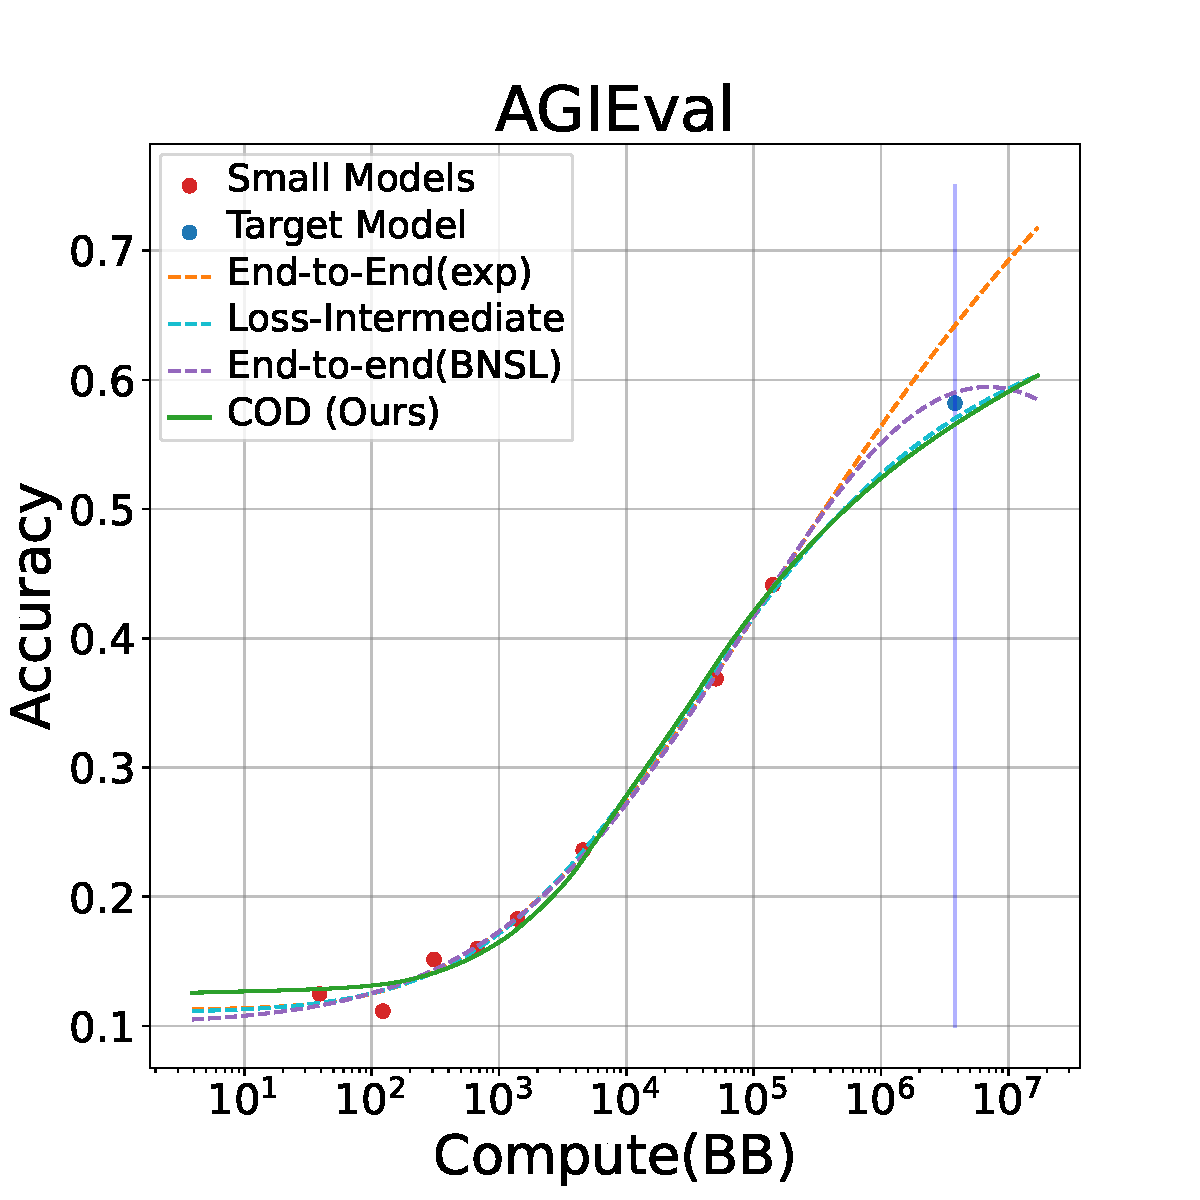
\includegraphics[width=\textwidth]{figures/experiments/perf_compute/AGIEVAL.pdf}  % 替换为实际文件名
    \end{minipage}
    \begin{minipage}{0.24\textwidth}
        \centering
        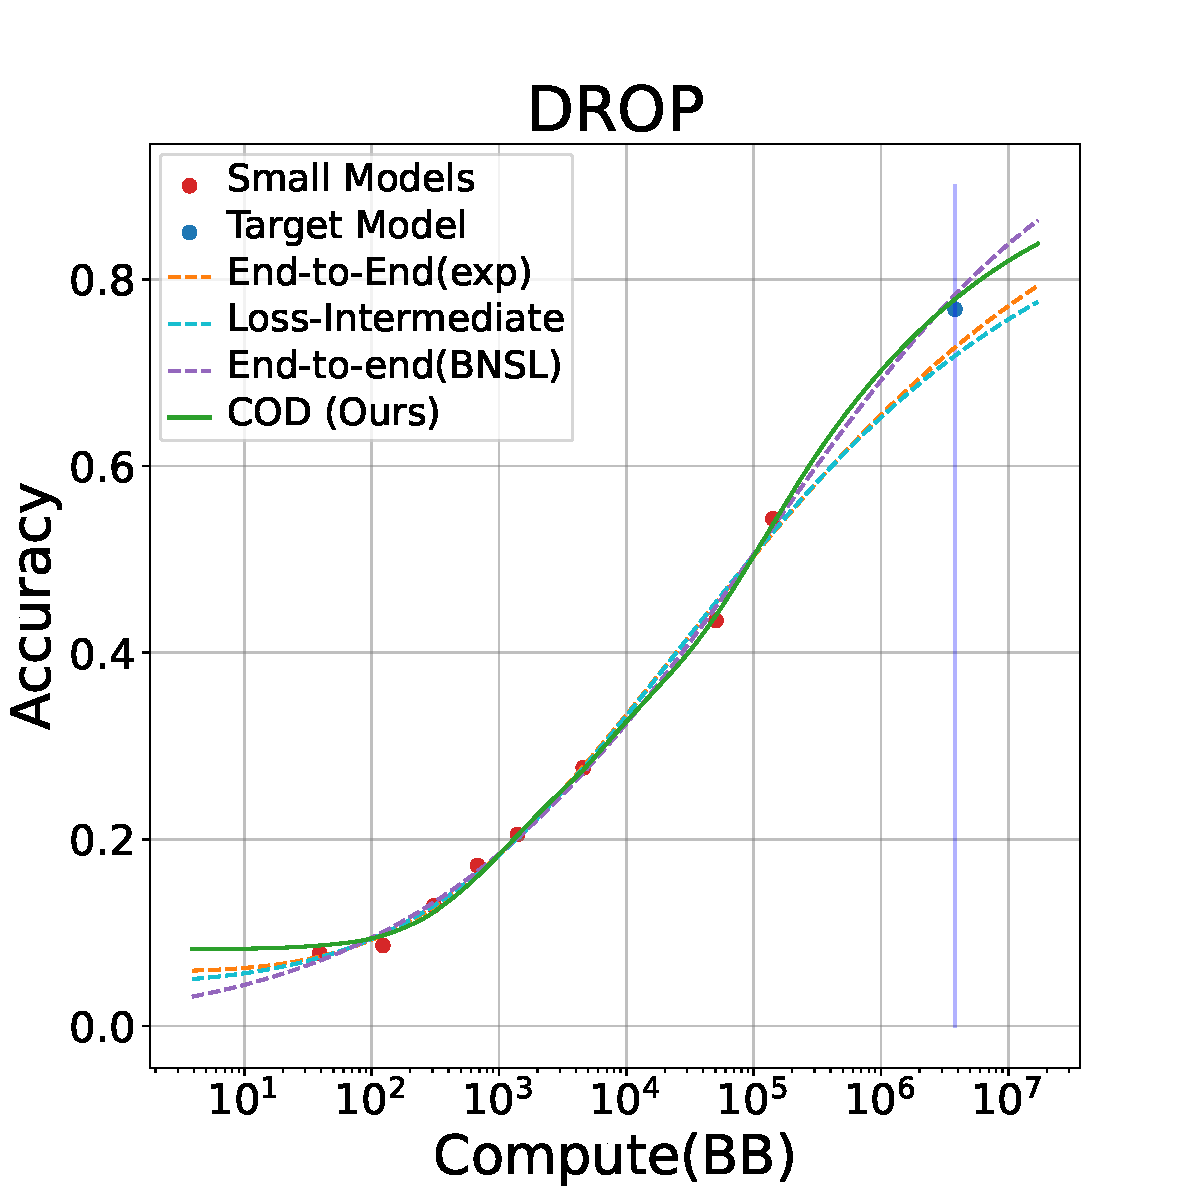
\includegraphics[width=\textwidth]{figures/experiments/perf_compute/DROP.pdf}  % 替换为实际文件名
    \end{minipage}
    \begin{minipage}{0.24\textwidth}
        \centering
        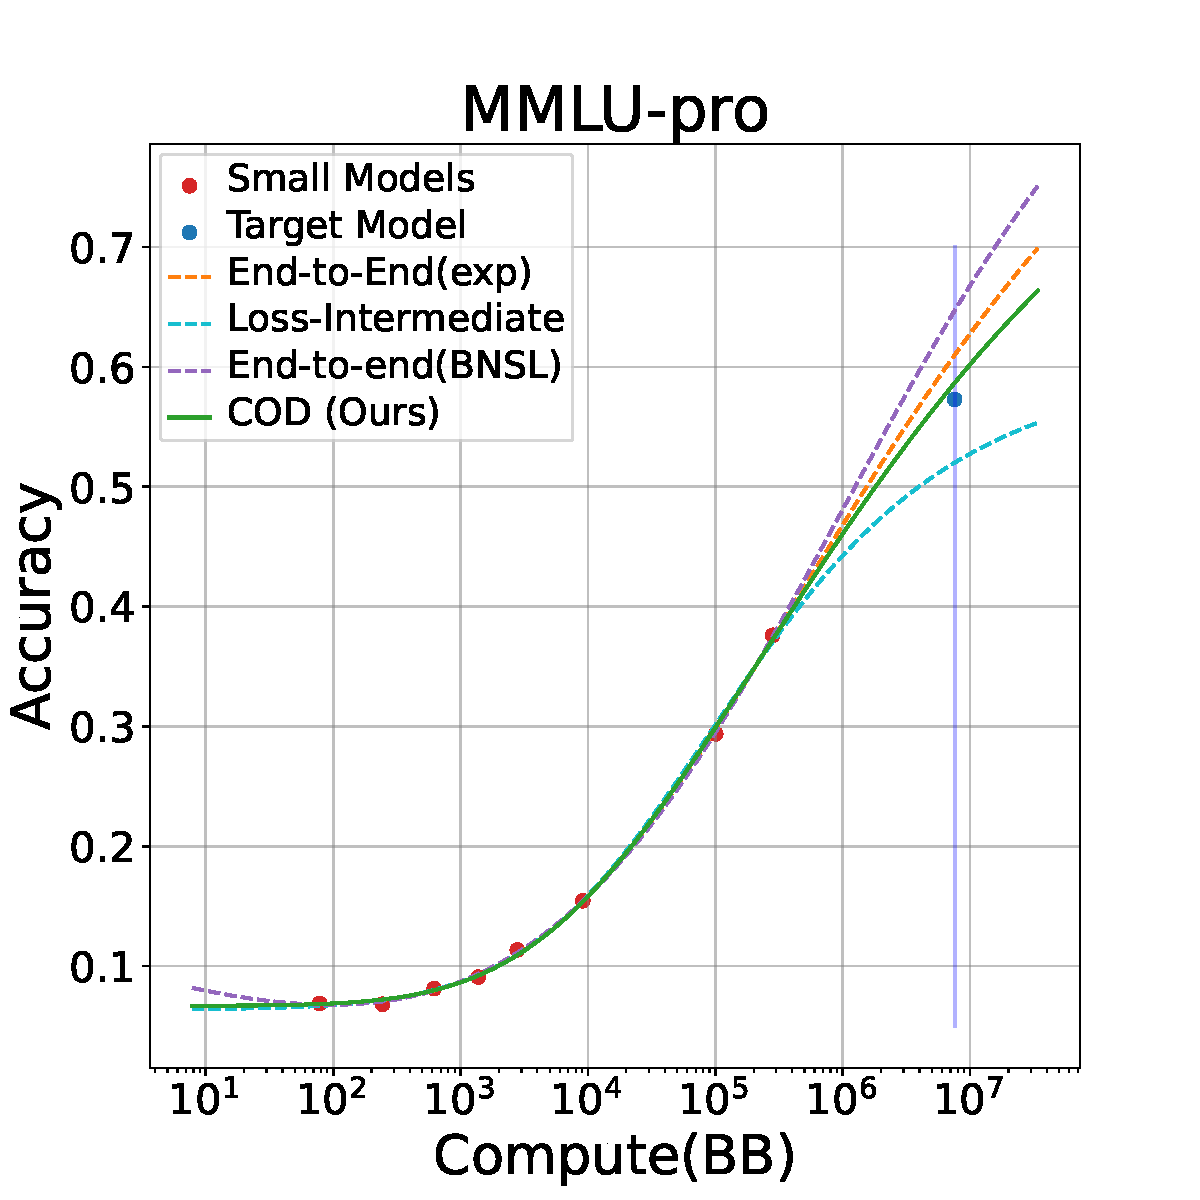
\includegraphics[width=\textwidth]{figures/experiments/perf_compute/MMLU-pro.pdf}  % 替换为实际文件名
    \end{minipage}
    \caption{Performance-compute relationship for different prediction methods on eight evaluation sets.}
    \label{fig:prediction_experiment_vis}
    % \vspace{-5pt}
\vspace{-10pt}

\end{figure}

\cref{fig:prediction_experiment_vis} visualizes the performance-compute relationships. The COD method does not merely extend the existing scaling trend; instead, it effectively predicts whether growth slowdown will occur subsequently and enables better estimation of the magnitude of curve bending.
On the BBH dataset, while End-to-end(exp) and loss-intermediate approaches perform comparably to COD, they show poor fitting on small-model data. COD reveals a more complex, better-fitted multi-phase trajectory. On MATH and MMLU-pro, where predicting accelerated growth versus plateaus is crucial, the loss-intermediate method underestimates model ceilings, and two end-to-end methods exceeds 3\% error. COD's superior performance stems from its nuanced analysis of difficulty distributions and scaling laws, allowing it to predict growth in challenging sets and capture diminishing returns in saturated sets.

\vspace{-5pt}
\subsection{Ablation Study}
To further validate the generalizability of the COD method, we conduct ablation experiments on \camera{different architecture}, clustering method and extrapolation function, while in the Appendix~\ref{sec:additional_ablation} we discuss ablation studies on the selection criteria for predictable subsets, interpolation mapping methods, and the influence of anchor point on predictions. We also examine its predictive capabilities after continual training with results documented in Appendix~\ref{sec:ppct}.

% \revise{\subsubsection{Prediction for a Medium-size Model}
% \label{sec:medium}
% The COD method is also effective for predicting the capabilities of medium-size language models. To demonstrate this, we conducted an experiment to predict the performance of a 12B model using source models ranging from 122M to 1.9B parameters. This setup maintains a similar ~6$\times$ parameter-size ratio as our main experiment (predicting 70B from models up to 12B).

% For this experiment, clustering relied exclusively on the passrate@100 data from the 122M to 1.9B source models to prevent data leakage from the target model. The results in~\cref{tab:12B_results} show that COD is more robust and less demanding on the size of source models compared to the baselines. For instance, the baseline methods perform poorly on the BBH benchmark, In contrast, COD accurately captures the trend of accuracy growth as compute increases and yields precise extrapolations. We will include a plot of this curve in the main text to visually demonstrate the clear advantage of COD.

% The prediction errors of all methods for the 12B model are significantly higher than those for the 70B model reported in~\cref{subsec:Prediction_Experiments}. Extrapolation accuracy improves when larger source models are employed for fitting, as a greater number of samples have ``emerged''. If the largest source model is excessively small, numerous samples remain ``unemerged'', resulting in substantial errors when extrapolating to a significantly larger model.}

% \begin{table*}[!t]
% \small
% \setlength{\tabcolsep}{1.8pt} % 保持原列间距设置
% \centering
% \caption{Absolute prediction error (\%) on evaluation sets for predicting the performance of the 12B model. Errors < 2\% are considered accurate (green), while errors > 5\% are considered invalid (red). $\downarrow$ indicates lower is better.}
% \begin{tabular}{c|c|cc|cc|cc|cc} % 列结构：任务/指标 | 真值 | 4组[Prediction|Error]
% \toprule
% \multirow{2}{*}{Task Sets/Metrics} & \multirow{2}{*}{Ground Truth} & \multicolumn{2}{c|}{\textbf{Loss-intermediate}} & \multicolumn{2}{c|}{\textbf{End-to-end}} & \multicolumn{2}{c|}{\textbf{BNSL}} & \multicolumn{2}{c}{\textbf{COD}} \\
% \cmidrule(lr){3-10} % 分隔线覆盖所有方法的Prediction-Error列
% & & Prediction & Error & Prediction & Error & Prediction & Error & Prediction & Error \\
% \toprule
% \multicolumn{10}{c}{\textbf{Overall Metrics}} \\ % 横向标题适配10列
% \midrule
% Mean & - & - & 14.92 & - & 10.52 & - & 17.42 & - & \textbf{4.68} \\
% Max & - & - & 23.82 & - & 24.43 & - & 28.26 & - & \textbf{10.39} \\
% \midrule
% \multicolumn{10}{c}{\textbf{Individual Task Sets}} \\ % 横向标题适配10列
% \midrule
% GSM8k & 70.47 & 60.86 & \redhl{9.61} & 63.66 & \redhl{6.81} & 80.99 & \redhl{10.52} & 60.08 & \redhl{10.39} \\
% MATH & 30.85 & 41.53 & \redhl{10.68} & 34.36 & 3.51 & 49.26 & \redhl{18.41} & 28.48 & 2.37 \\
% BBH & 60.76 & 36.94 & \redhl{23.82} & 36.33 & \redhl{24.43} & 36.10 & \redhl{24.66} & 57.751 & 3.05 \\
% TriviaQA & 58.84 & 68.42 & \redhl{9.57} & 59.88 & \greenhl{1.04} & 87.10 & \redhl{28.26} & 57.92 & \greenhl{0.93} \\
% MBPP & 47.80 & 28.53 & \redhl{19.27} & 36.51 & \redhl{11.29} & 27.95 & \redhl{19.85} & 44.50 & 3.30 \\
% AGIEval & 44.13 & 33.91 & \redhl{10.22} & 35.40 & \redhl{8.74} & 34.12 & \redhl{10.01} & 47.53 & 3.40 \\
% DROP & 54.35 & 35.05 & \redhl{19.30} & 37.19 & \redhl{17.16} & 36.73 & \redhl{17.62} & 63.50 & \redhl{9.14} \\
% MMLU-pro & 37.60 & 20.74 & \redhl{16.86} & 26.41 & \redhl{11.20} & 27.59 & \redhl{10.01} & 42.42 & 4.82 \\
% \bottomrule
% \end{tabular}
% \label{tab:12B_results}
% % \vspace{-10pt}
% \end{table*}

\subsubsection{\camera{Prediction on MoE models}}
% COD方法依赖于样本粒度的重复评测以及聚类，带来了额外的复杂度与算力开销。然而难度特征是属于题目本身与模型相对独立，聚类结果应该可以在不同模型族的预测任务中进行服用。我们下面验证利用Dense小模型获得预测结果可以外推到一系列MoE模型上。
% \camera{The COD approach relies on repeated sample-level evaluation and clustering, which introduces additional complexity and computational overhead. However, difficulty characteristics are inherent to the tasks themselves and are relatively model-agnostic, so the clustering results should be reusable across prediction tasks of different model families. Below, we verify that prediction results derived from small dense models can be extrapolated to a range of MoE models.
% To verify the robustness of the clustering results, we perform one-shot evaluation across benchmarks on a 32B activated-parameter MoE model, using the clustering results obtained from pre-trained dense models. Comparative results are shown in \cref{tab:MoE_exp}.}
% 可以看出在夸模型结构的预测上，COD方法取得了最优的平均预测误差，说明其难度特征与类簇在不同模型族之间具有一定迁移效果。但预测精度相比预测Dense模型有所下降，估计难度特征的模型与用于预测外推的模型保持一致可以最小化类内任务的Scaling差异，并取得更好的预估结果。
% \camera{It can be seen that the COD method achieves the best average prediction error in cross-architecture prediction, indicating that its difficulty characteristics and clusters have a certain transferability across different model families.
% However, the prediction accuracy decreases compared with forecasting on dense models.
% We conjecture that keeping the model used for estimating difficulty characteristics consistent with the model for extrapolation can minimize the scaling differences of within-cluster tasks and yield better estimation results.}

\camera{
COD relies on repeated sample-level evaluation and clustering, introducing additional computational overhead. 
However, difficulty characteristics are task-inherent and largely model-agnostic, suggesting that the resulting clusters can generalize across model families. 

To test this transferability, we conduct one-shot evaluations on a 32B activated-parameter MoE model using clusters derived from pre-trained dense models. Results in \cref{tab:MoE_exp} show that COD achieves the lowest average prediction error in cross-architecture extrapolation, indicating that its difficulty features and clusters transfer effectively across model families. 
Nevertheless, prediction accuracy is lower than in dense-to-dense extrapolation. We hypothesize that aligning the model used for difficulty estimation with the target model for extrapolation reduces intra-cluster scaling discrepancies and improves prediction accuracy.
}
\begin{table*}[!t]
\small
\setlength{\tabcolsep}{1.8pt} % Keep this if column spacing is critical
\centering
\caption{Absolute prediction error (\%) on evaluation sets for predicting the performance of the 32B MoE model. Errors < 2\% are considered accurate (green), while errors > 5\% are considered invalid (red). $\downarrow$ indicates lower is better.}
\begin{tabular}{c|cc|ccccccc}
\toprule
\multirow{2}{*}{Method} & \multicolumn{2}{c|}{Overall Metrics} & \multicolumn{7}{c}{Individual Task Sets} \\
\cmidrule(lr){2-3} \cmidrule(lr){4-10}
& Mean$\downarrow$ & Max$\downarrow$ & GSM8k & MATH & BBH & TriviaQA & MBPP & AGIEval & DROP \\
\midrule
Loss-intermediate & 3.65 & \textbf{7.24} & \greenhl{0.45} & \greenhl{0.62} & 4.48 & \greenhl{0.36} & 4.92 & \redhl{7.24} & 4.55 \\
End-to-end(exp) & 3.95 & 7.86 & 2.75 & \greenhl{1.43} & 3.88 & \greenhl{1.72} & \redhl{7.86} & \redhl{7.79} & 2.21 \\
% End-to-end(BNSL) &  &  &  &  &  &  &  &  &  \\
\midrule
COD (Complete) & \textbf{3.11} & 8.11 & \greenhl{0.54} & \greenhl{1.72} & \redhl{5.29} & \greenhl{0.27} & \redhl{8.11} & \greenhl{0.57} & \redhl{5.24} \\
\bottomrule
\end{tabular}
\label{tab:MoE_exp}
\vspace{-8pt}
\end{table*}

\subsubsection{Comparison of Clustering Methods}
\label{sec:clustering_ablation}

We assess the impact of different clustering algorithms on prediction accuracy. The goal is to achieve tight intra-cluster difficulty similarity (low average distance to center) while maintaining cluster stability (min. 10 samples/cluster). We compare our Improved-MeanShift with DBScan, MeanShift, and K-Means. For K-Means, we adjust it to approximate our goals: (1) search for $k$ yielding min. cluster sizes $\approx 10$; (2) treat samples outside a radius (e.g., 2$\times$ average intra-cluster distance) from any cluster center as outliers, and we ensure clusters don't drop below 10 samples. We term this "Improved-KMeans" for this comparison. Clustering quality is measured by Intra-cluster Average Distance (IAD) and Outlier Rate (OR). Prediction benefits are measured by Extrapolation Error (EE) on the predictable subset and Final prediction Error (FE) on the full evalset. (\cref{tab:clustering_prederror}).

\begin{table*}[!t]
\centering
\scriptsize % 使用更小的字体 (比 footnotesize 更小)
\caption{Clustering performance across different algorithms on metrics including IAD (Intra-cluster Average Distance$\downarrow$), OR (Outlier Rate \%), EE (Extrapolation Error$\downarrow$), FE (Final Prediction Error$\downarrow$). The bottom lines show the mean and max EE and FE across evalsets.}
\setlength{\tabcolsep}{1.5pt} % 进一步减小列间距
\resizebox{\textwidth}{!}{% 自适应页面宽度
\begin{tabular}{l|cccc|cccc|cccc|cccc|cccc}
\toprule
\multirow{2}{*}{Dataset} & \multicolumn{4}{c|}{KMeans} & \multicolumn{4}{c|}{DBScan} & \multicolumn{4}{c|}{MeanShift} & \multicolumn{4}{c|}{Improved-KMeans} & \multicolumn{4}{c}{Improved-MeanShift} \\
\cmidrule(lr){2-5} \cmidrule(lr){6-9} \cmidrule(lr){10-13} \cmidrule(lr){14-17} \cmidrule(lr){18-21}
& IAD & OR & \textbf{EE} & \textbf{FE} & IAD & OR & \textbf{EE} & \textbf{FE} & IAD & OR & \textbf{EE} & \textbf{FE} & IAD & OR & \textbf{EE} & \textbf{FE} & IAD & OR & \textbf{EE} & \textbf{FE} \\
\midrule

GSM8k    & 0.22 & - & \textbf{0.01} & \textbf{0.00} & 0.51 & 0.53 & 4.08 & 4.12 & 0.29 & 0.61 & 0.67 & 0.74 & \textbf{0.13} & 2.73 & 3.92 & 4.08 & 0.16 & 7.05 & 0.31 & 2.68 \\
MATH     & 0.22 & - & 2.62 & 2.34 & 0.48 & 0.68 & 4.38 & 4.16 & 0.21 & 1.44 & 2.55 & 2.26 & \textbf{0.09} & 2.22 & \textbf{0.81} & \textbf{0.51} & 0.11 & 6.26 & 0.84 & 0.79 \\
BBH      & 0.63 & - & 8.16 & 8.99 & 0.71 & 18.92 & 3.53 & 4.36 & 0.27 & 20.72 & 2.12 & 0.65 & \textbf{0.20} & 37.23 & \textbf{0.02} & 2.17 & 0.21 & 33.58 & 0.54 & \textbf{0.47} \\
TriviaQA & 0.44 & - & 2.97 & 2.46 & 0.70 & 6.38 & \textbf{1.11} & \textbf{0.81} & 0.25 & 6.77 & 3.64 & 4.90 & \textbf{0.12} & 11.97 & 1.18 & 1.12 & 0.19 & 11.54 & 1.56 & 1.97 \\
MBPP     & 0.34 & - & 2.53 & 2.67 & 0.51 & 12.80 & \textbf{1.57} & 1.41 & 0.22 & 15.60 & 2.40 & \textbf{1.22} & \textbf{0.17} & 19.40 & 2.39 & 3.25 & \textbf{0.17} & 21.60 & 1.61 & 2.42 \\
AGIEval  & 0.46 & - & 2.61 & 2.68 & 0.56 & 3.67 & 6.43 & 6.27 & 0.29 & 2.99 & 2.63 & 3.23 & \textbf{0.15} & 7.60 & 5.96 & 5.56 & 0.21 & 11.50 & \textbf{1.11} & \textbf{1.64} \\
DROP     & 0.56 & - & 1.66 & 1.64 & 0.67 & 11.08 & 3.03 & 2.66 & 0.25 & 11.81 & 4.18 & 4.00 & \textbf{0.14} & 21.42 & 3.99 & 5.24 & 0.20 & 19.88 & \textbf{1.44} & \textbf{1.05} \\
MMLU-pro & 0.32 & - & 3.69 & 3.69 & 0.42 & 0.56 & 3.72 & 3.69 & 0.29 & 0.39 & 3.15 & 3.08 & \textbf{0.16} & 2.85 & \textbf{0.56} & \textbf{0.61} & 0.22 & 4.40 & 1.26 & 1.39 \\
\midrule
\textbf{Mean} & - & - & 3.03 & 3.06 & - & - & 3.48 & 6.43 & - & - & 2.67 & 2.51 & - & - & 2.35 & 2.82 & - & - & \textbf{1.08} & \textbf{1.55} \\
\textbf{Max}  & - & - & 8.16 & 8.99 & - & - & 4.38 & 4.36 & - & - & 4.18 & 4.90 & - & - & 5.96 & 5.56 & - & - & \textbf{1.61} & \textbf{2.68} \\
\bottomrule
\end{tabular}
} % 结束 resizebox
\label{tab:clustering_prederror}
\vspace{-5pt}
\end{table*}


\cref{tab:clustering_prederror} shows Improved-KMeans and Improved-MeanShift yield better clustering (lower IAD) due to their intra-cluster distance constraints. The results also confirm these methods lead to lower EE and FE. Although Improved-KMeans has the best IAD,  it performs poorly on GSM8k, AGIEval, and DROP. This is likely because K-Means requires pre-specifying $k$, and our search for $k$ can be unstable, leading to large errors on some sets. In contrast, our Improved-MeanShift, which automatically determines $k$ based on distance constraints, offers more stable clustering and the lowest maximum prediction error.

\subsubsection{Different Extrapolation Formulas}
\label{sec:ablation_extrapolation}
\begin{table*}[!t]
\centering
\small
\caption{Ablation study on extrapolation formulas. EE, TR, FE shown for BBH, MATH, MMLU-pro.}
\begin{tabular}{c|ccc|ccc|ccc}
\toprule
\multirow{2}{*}{Method} & \multicolumn{3}{c}{BBH} & \multicolumn{3}{c}{MATH} & \multicolumn{3}{c}{MMLU-pro} \\
\cmidrule(lr){2-4} \cmidrule(lr){5-7} \cmidrule(lr){8-10}
& EE$\downarrow$ & TR(\%) & FE$\downarrow$ & EE$\downarrow$ & TR(\%) & FE$\downarrow$ & EE$\downarrow$ & TR(\%) & FE$\downarrow$ \\
\midrule
w/o Random Guess ($f_1$) & 10.40 & 48.29 & 11.65 & 3.96 & 76.82 & 3.22 & 4.40 & 95.05 & 4.32 \\
w/o Constant c ($f_2$) & 2.15 & 57.21 & 4.10 & 1.50 & 76.82 & 1.36 & 3.85 & 95.60 & 3.96 \\
Direct Power Law ($f_3$) & 8.90 & 49.05 & 8.85 & 3.33 & 76.82 & 2.70 & 4.30 & 95.15 & 4.20 \\
Ours ($f$) & \textbf{0.54} & 53.39 & \textbf{0.47} & \textbf{0.84} & 76.82 & \textbf{0.79} & \textbf{1.26} & 94.38 & \textbf{1.39} \\
\bottomrule
\end{tabular}
\label{tab:ablation_results}
\vspace{-5pt}
\end{table*}
We ablate our proposed fitting formula $f(C)=g+(1-g) \cdot e^{-aC^{-b}-c}$ (Ours) by removing or modifying components:
(1) $f_1(C)=e^{-aC^{-b}-c}$ (w/o random guess);
(2) $f_2(C)=g+(1-g) \cdot e^{-aC^{-b}}$ (w/o constant $c$);
(3) $f_3(C) = e^{-aC^{-b}}$ (Direct Power Law~\citep{hu2023predicting}).
\cref{tab:ablation_results} shows Extrapolation Error (EE), Task Ratio of predictable subset (TR), and Final prediction Error (FE).
Our proposed formula $f$ consistently achieves the lowest EE and FE. $f_1$ struggles with finite-answer tasks where small models have non-zero scores. $f_2$ inaccurately assumes perfect scores are attainable, ignoring data limitations and task ambiguities. The direct power law ($f_3$) fails to model the 0-1 metric range and the varying difficulty of improvement near random guess and saturation. \camera{The weak correlation between TR and prediction error demonstrates the robustness of our COD framework: even when the proportion of the predictable subset is low due to non-emergent tasks, the performance of non-extrapolatable tasks can still be accurately inferred through the proposed mapping function.}
% TR's minor influence on prediction error suggests robustness; even with low TR due to non-emergent tasks, their performance can be largely predicted via mapping.